\subsection{Verification of the analytic constants}\label{sec:constants}
Each constant in Theorem~\ref{thm:main} can be verified separately. This section gives the
conditional variance and the direction of the mean; the window width, dynamic variance, and
selection strength are verified in Appendix~\ref{app:exp-constants}, and cross-validation
across independent realizations appears in Appendix~\ref{app:exp-indep}.

\emph{Conditional variance.} At $k=6$, $M=16384$, and failure probability $0.10$, the
measured value is $0.9604$, and the selection law gives $0.9600$. At $k=3$, on the
low-failure-probability grid points $M=65536$ and $262144$, the measured values are $0.8989$
and $0.8987$, and the theoretical value is $0.8971$.

\emph{Sign change.} At every failure-probability level and every $M$, the one-sided
conditional mean is negative for $k=5,6$ and positive for $k=3$. At $M=262144$, the largest
deviation between measurement and prediction is $1.4$ standard errors.

Figure~\ref{fig:selection} summarizes the 444 configurations and sign composition rows with
$M\ge4096$ ($k=3$--$6$, $M=4096$--$262144$); the theoretical curves use only the analytic
constants $\eta_k$. The horizontal axis is the measured failure probability, equivalently
comparing on the empirical coordinate $z_{\rm emp}=\Phi^{-1}(\widehat p_F)$. Thus this figure
verifies the conditional distribution itself; the finite-size shift of the threshold center is
handled separately in Section~\ref{sec:threshold}. When all signs are equal, the conditional
means of all four $k$ lie on the curve $-\eta_kA(z_{\rm emp})$, and the direction reverses
between $k=4$ and $k=5$. After dividing the conditional mean by $-A(z_{\rm emp})$, all sign
compositions lie on a straight line through the origin with slope $\eta_k$, and the balanced
sign composition returns to the origin; this panel verifies both the value of $\eta_k$ and its
decay in $\rho^2$. For the all-equal-sign rows, the median relative error at $k=3$ decreases
from $4.7\%$ at $M=4096$ to $0.8\%$ at $M=262144$, and at $k=5$ it does not exceed $0.5\%$ at
any size.
\begin{figure}[!htbp]
\centering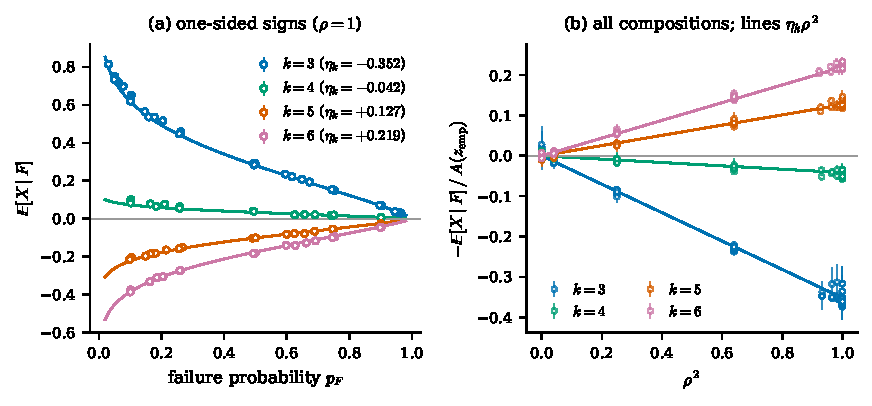
\includegraphics[width=\linewidth]{figures/fig-selection-law.pdf}
\caption{Failure conditional mean versus the analytic prediction ($M\ge4096$). (a) all signs
equal, curve $-\eta_kA(\Phi^{-1}(p_F))$; (b) all sign compositions, line $\eta_k\rho^2$.
}
\label{fig:selection}
\end{figure}
